\chapter{Interval graphs}
\label{chap:interval}

\begin{fquote}[Robert Callaghan][Big Hero 6]
  If you like easy, my program isn’t for you. Nothing great comes from easy.
\end{fquote}


The goal of this chapter is to present the family of classes of interval graphs that are related to the class of thin strip graphs. We introduce the class of interval graphs, which is
 one of the most used classes of intersection graphs. There are multiple types of
 interval graphs and those that are the most relevant for the thesis are going to be defined below.

 First, we recall the basic definition of an interval graphs and their multiple characterizations. Also, we present unit interval graphs, where we see their characterization and complexity such as Robert's characterization \cite{roberts1968representations}. Then, we see some characterizations such as Joos's paper about mixed unit interval graphs \cite{joosCharacterizationMixedUnit2013} and the paper from Hayashi \textit{et al.} \cite{hayashiThinStripGraphs2017} where the unfettered unit interval graphs are defined and also characterized as well as some equivalences with \emph{unit disk graphs} are presented. Also, the complexity of the recognition for each one of the classes presented will be discussed.

\section{Interval graphs}

First we present the main characterizations of interval graphs. In the next sections we present some other subclasses of interval graphs that will help us characterize the thin strip graphs on Chapter \ref{chap:thinDef}. There are multiple characterizations of interval graphs that are equivalent, in this thesis we present Gilmore and Hoffman's characterization described in Theorem \ref{theo:intvalChord}. From this theorem it is clear that \textit{IG} class is a subclass of the \textit{CO-CO} class.

\begin{theorem}[Gilmore and Hoffman \cite{gilmoreCharacterizationComparabilityGraphs1964}]
  \label{theo:intvalChord}
  $G$ is an interval graph if and only if $G$ does not contain $C_4$ as an induced subgraph and $\overline{G}$ can be ordered partially, in other words, $\overline{G}$ is a comparability graph.
\end{theorem}

The first interesting subclass of IG is the class of \emph{unit interval graphs} which is defined by the interval graphs that have intervals with the same length (or equal to one). This class of graphs is equivalent to the class of \emph{proper interval graph} which is the class of intervals where no interval is a strict subset of another. This statement is powerful because the study of unit interval graphs can be more confortable because of the simplicity of its definition and characterization as seen in Theorem \ref{theo:k_13}.

\begin{theorem}[Roberts \cite{roberts1968representations}]
  \label{theo:k_13}
  An interval graph is a unit interval graph if and only if it has no induced subgraph $K_{1,3}$ \footnote{$K_{1,3}$ is also called \emph{claw}.}.
\end{theorem}

In terms of recognition, interval graphs as long as unit interval graphs can be recognized in \emph{linear time}. Interval graph linear time recognition was discovered by Booth \textit{et al.} by doing so with a \emph{breadth-first search} \cite{boothTestingConsecutiveOnes1976}. UIG recognition has also been proven to be linear \cite{corneil1987extensions}.

\section{Mixed unit interval graphs}
\label{sec:muig}

We can define a new class of graphs that is related to UIG by its definition. This class is closely related to thin strip graphs as we will see in Chapter \ref{chap:thinDef}. \emph{Mixed unit interval graphs} are graphs where the intervals have the same size as the unit interval graphs. However, in this class, the endpoints of the intervals can be open or closed - or one of each.

Formally, MUIG is defined by using the next classes of graphs:

$$\mathcal{U}^{++} = \{[x,y] : x,y \in \mathbb{R}, x\leq y\}$$
$$\mathcal{U}^{--} = \{(x,y) : x,y \in \mathbb{R}, x\leq y\}$$
$$\mathcal{U}^{+-} = \{[x,y) : x,y \in \mathbb{R}, x\leq y\}$$
$$\mathcal{U}^{-+} = \{(x,y] : x,y \in \mathbb{R}, x\leq y\}$$

where $\mathcal{U}^{xx}$ is the class of unit interval graphs where its intervals can be open or closed depending on their sign. For exemple, $\mathcal{U}^{++} = \text{UIG}$.

Dourado, by defining these classes of unit interval graphs with open/closed intervals also found that, for unit interval graphs, it does not matter if the endpoints are open, closed, or closed open (Theorem \ref{theo:douradoEquiv}).

\begin{theorem}[Dourado et al. \cite{DOURADO20123357}]
  \label{theo:douradoEquiv}
  The classes of the graphs $\mathcal{U}^{--}$, $\mathcal{U}^{++}$,
  $\mathcal{U}^{-+}$, $\mathcal{U}^{+-}$, and  $\mathcal{U}^{-+} \bigcup
  \mathcal{U}^{+-}$ are the same.
\end{theorem}

\begin{figure}
\centering
\begin{scaletikzpicturetowidth}{\textwidth}
\begin{tikzpicture}[scale=1.5]

  \draw[{(-)}] (-1,-0.5) -- (0,-0.5);
  \draw[color=black] (-0.4845,-0.8507) node {$v_4$};
  \draw[{[-}] (0,-1.5) -- (1,-1.5);
  \draw[color=black] (0.5023,-1.3568) node {$v_3$};
  \draw[{-]}] (-2,-1.5) -- (-1,-1.5);
  \draw[color=black] (-0.4899,-0.3468) node {$v_2$};
  \draw[{[-]}] (-1,-1) -- (0,-1);
  \draw[color=black] (-1.4962,-1.3536) node {$v_1$};

  \node[draw,circle,inner sep=2pt,fill,label distance=1cm] (v1) at (-4,-0.25) {};
  \draw[color=black] (-4,0) node {$v_4$};
  \node[draw,circle,inner sep=2pt,fill,label distance=1cm] (v3) at (-4,-1.25) {};
  \draw[color=black] (-4,-1.5) node {$v_2$};
  \node[draw,circle,inner sep=2pt,fill,label distance=1cm] (v2) at (-5,-1.25) {};
  \draw[color=black] (-3,-1.5) node {$v_3$};
  \node[draw,circle,inner sep=2pt,fill,label distance=1cm] (v4) at (-3,-1.25) {};
  \draw[color=black] (-5,-1.5) node {$v_1$};
  \draw  (v1) edge (v2);
  \draw  (v1) edge (v3);
  \draw  (v1) edge (v4);

\end{tikzpicture}
\end{scaletikzpicturetowidth}

\caption{Representation of $K_{1,3}$ as a MUIG.}
\label{fig:muigK13}
\end{figure}

However, MUIG is defined as $\mathcal{U}^{++} \bigcup \mathcal{U}^{--} \bigcup \mathcal{U}^{+-} \bigcup \mathcal{U}^{-+}$ which is also denoted as $\mathcal{U}$. In this case it is clear that this class is not equivalent to UIG. As we have seen in Theorem \ref{theo:k_13}, a UIG can be seen as a $K_{1,3}$-free IG. Nevertheless, MUIG can accept this graph as seen in Proposition \ref{prop:k_13MUIG}.

\begin{prop}[Dourado \textit{et al.} \cite{douradoMixedUnitInterval2012}]
  \label{prop:k_13MUIG}
  MUIG has a $K_{1,3}$ representation. Also, for every MUIG representation $\phi : V(K_{1,3}) \to \mathcal{U}$ such that $\phi(V(K_{1,3}))$ contains:

  \begin{itemize}
    \item $a = [x, x+1]$
    \item $b = (x, x+1)$
    \item $c = [x+1, x+2]$ or $[x+1, x+2)$
    \item $d = [x-1, x]$ or $[x-1, x)$
  \end{itemize}
\end{prop}

\begin{proof}
Let $\phi : V(K_{1,3}) \to \mathcal{U}$ be the representation of $K_{1,3}$ as a mixed unit interval intersection diagram as illustrated in Figure \ref{fig:muigK13}. Let $V(K_{1,3}) = \{v_1, v_2, v_3, v_4\}$ and $E(K_{1,3}) = \{v_1v_4, v_2v_4, v_3v_4\}$. Let $x(v_1) = I(v_1) \cap I(v_4)$, $x(v_2) = I(v_2) \cap I(v_4)$ and $x(v_3) = I(v_3) \cap I(v_4)$. Because $v_1, v_2$ and $v_3$ are not adjacent, we can assume that $x(v_1) < x(v_2) < x(v_3)$. Since $x(v_1) \in I(v_4)$ and $x(v_3) \in I(v_4)$, then $x(v_3) - x(v_1) \leqslant 1$. Since $I(v_1), I(v_2)$ and $I(v_3)$ are disjoint, $I(v_2)$ must be a proper subset of $(x(v_1), x(v_3))$. Since $I(v_2)$ is a mixed unit interval, then it implies that $x(v_3) = x(v_1) + 1$, $I(v_2) = (x(v_1), x(v_1+1))$, $I(v_4) = [x(v_1), x(v_1)+1]$, $I(v_1) = \{(x(v_1) -1, x(v_1)], [x(v_1) -1, x(v_1)]\}$ and $I(v_3) = \{[x(v_3) -1, x(v_3)), [x(v_3) -1, x(v_3)]\}$.
\end{proof}

\begin{theorem}[Dourado \textit{et al.} \cite{douradoMixedUnitInterval2012}]
  $\text{UIG} \subsetneq \text{MUIG}$.
\end{theorem}

\begin{proof}
  The strict inclusion is straightforward: we know that $\text{UIG} = \mathcal{U}^{++} \subset MUIG$ by definition. For the inequality, we prove it by Proposition \ref{prop:k_13MUIG}, as $K_{1,3}$ is not realizable in UIG.
\end{proof}

Nevertheless, MUIG still shares some properties with UIG. In the previous section we mentioned that the class of unit interval graphs is the same as the class of proper interval graphs. In our case, mixed unit interval graphs is also exactly the same as the mixed proper interval graphs -- where no mixed interval can be a proper subset of another one.

\begin{theorem}
  For a graph $G$, the following two statements are equivalent.
  \begin{itemize}
    \item $G$ is a mixed proper interval graph.
    \item $G$ is a mixed unit interval graph.
  \end{itemize}
\end{theorem}

Shuchat \textit{et al.} \cite{shuchatUnitMixedInterval2014} describe an algorithm to recognize mixed unit interval graphs in polynomial time with a characterization. Proof and details about the algorithm will not be provided but we encourage the reading of their paper.

\begin{theorem}[Schuchat et al. \cite{shuchatUnitMixedInterval2014}]
 The MUIG recognition problem is in $\mathcal{P}$. Moreover, there is an algorithm that solves it in $\mathcal{O}(|V|^2)$ for $V$ the vertex set of a graph.
\end{theorem}


\subsection{Characterization}
\label{sec:muig_char}

A complete characterization by induced forbidden subgraphs have been found independently by A. Schuchat et al. \cite{shuchatUnitMixedInterval2014a} and F. Joos \cite{joosCharacterizationMixedUnit2013}. In this section we will present briefly the characterization of MUIG given by Joos with forbidden subgraphs. We will also review each one of these forbidden subgraphs and discuss the properties compared of one of them that will be relevant in the next chapter. However, the proof of this characterization will not be given in this thesis because of its length. His work follows Dourado \textit{et al.} \cite{douradoMixedUnitInterval2012} where they characterized \emph{diamond-free} mixed unit interval graphs.

\begin{theorem}[Joos \cite{joosCharacterizationMixedUnit2013}]
  $G$ is a MUIG if and only if it is a $\{F\}\cup\mathcal{R}\cup\mathcal{S}\cup\mathcal{S''}\cup\mathcal{T}$-free interval graph.
\end{theorem}

The forbidden families can be seen in Figures \ref{fig:graphsR}, \ref{fig:graphsS}, \ref{fig:graphsSS}, \ref{fig:graphF}, \ref{fig:graphsT}. You can notive that, without including $F$, every family of forbidden graphs of MUIG is infinite and is defined recursively by its predecessor. Our only goal in this section is to focus in the properties of $\mathcal{R}$ because, as we will see in Chapter \ref{chap:thinDef}, it is the only forbidden graph family for MUIG that is also forbidden for thin strip graphs.

We know that $\mathcal{R}$ is a family of forbidden subgraph for mixed unit interval graphs. If we look up in the graph classes hierarchy \ref{fig:hierarchyMUIG} we find that MUIG $\subsetneq$ CO-CO. The first step to see if $\mathcal{R}$ is a family of proper forbidden subgraph for MUIG is to prove if $\mathcal{R} \subsetneq$ CO-CO. In the first place, we present a characterization of cocomparability graphs.

\begin{theorem}[Damaschke \cite{damaschkeDistancesCocomparabilityGraphs1992}]
  \label{theo:spanning}
  A graph $G$ is a co-comparability graph if and only if it has a spanning order.
\end{theorem}


\begin{figure}
\begin{center}
\begin{scaletikzpicturetowidth}{\textwidth}
\begin{tikzpicture}[scale=1]
  \node (1) [draw, rounded rectangle] {co-comparability graphs};
  \node (2) [below=of 1, draw, rounded rectangle] {mixed unit interval graphs};
  \node (3) [below=of 2, draw, rounded rectangle] {unit interval graphs};
  \draw[<-] (1) edge (2) (2) edge (3);
\end{tikzpicture}
\end{scaletikzpicturetowidth}
\end{center}
\caption{The hierarchy of the classes between \emph{UIG} and \emph{CO-CO}. The arrows represent a relation of $\subsetneq$.}\label{fig:hierarchyMUIG}
\end{figure}


\begin{figure}[H]
\begin{center}
  \begin{scaletikzpicturetowidth}{\textwidth}
  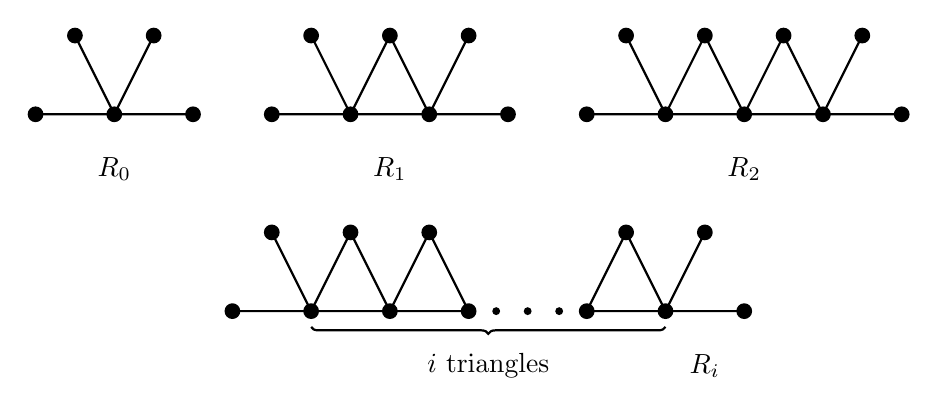
\begin{tikzpicture}[scale=1]
\def\ver{0.1} %size of a vertex
\def\x{1}

\def\xa{0.5}
\def\ya{0}

\def\xb{4}
\def\yb{0}

\def\xc{8}
\def\yc{0}

\def\xd{3.5}
\def\yd{-2.5}


%graph R_0
\path[fill] (\xa+0.5,\ya) circle (\ver);
\path[fill] (\xa+1,\ya+1) circle (\ver);
\path[fill] (\xa+2,\ya+1) circle (\ver);
\path[fill] (\xa+2.5,\ya) circle (\ver);
\path[fill] (\xa+1.5,\ya) circle (\ver);

\draw[thick] (\xa+0.5,\ya)--(\xa+1.5,\ya)--(\xa+1,\ya+1)
(\xa+2,\ya+1)--(\xa+1.5,\ya)--(\xa+2.5,\ya);

\node (1) at (\xa+1.5,\ya-0.7) {$R_0$};

%graph R_1
\path[fill] (\xb,\yb) circle (\ver);
\path[fill] (\xb+1,\yb) circle (\ver);
\path[fill] (\xb+2,\yb) circle (\ver);
\path[fill] (\xb+3,\yb) circle (\ver);
\path[fill] (\xb+0.5,\yb+1) circle (\ver);
\path[fill] (\xb+1.5,\yb+1) circle (\ver);
\path[fill] (\xb+2.5,\yb+1) circle (\ver);

\draw[thick] (\xb,\yb)--(\xb+1,\yb)--(\xb+2,\yb)--(\xb+3,\yb)
(\xb+0.5,\yb+1)--(\xb+1,\yb)--(\xb+1.5,\yb+1)--(\xb+2,\yb)--(\xb+2.5,\yb+1);

\node (1) at (\xb+1.5,\yb-0.7) {$R_1$};


%graph R_2
\path[fill] (\xc,\yc) circle (\ver);
\path[fill] (\xc+1,\yc) circle (\ver);
\path[fill] (\xc+2,\yc) circle (\ver);
\path[fill] (\xc+3,\yc) circle (\ver);
\path[fill] (\xc+4,\yc) circle (\ver);
\path[fill] (\xc+0.5,\yc+1) circle (\ver);
\path[fill] (\xc+1.5,\yc+1) circle (\ver);
\path[fill] (\xc+2.5,\yc+1) circle (\ver);
\path[fill] (\xc+3.5,\yc+1) circle (\ver);

\draw[thick] (\xc,\yc)--(\xc+1,\yc)--(\xc+2,\yc)--(\xc+3,\yc)--(\xc+4,\yc)
(\xc+0.5,\yc+1)--(\xc+1,\yc)--(\xc+1.5,\yc+1)--(\xc+2,\yc)--(\xc+2.5,\yc+1)--(\xc+3,\yc)--(\xc+3.5,\yc+1);

\node (1) at (\xc+2,\yc-0.7) {$R_2$};

%graph R_i
\path[fill] (\xd,\yd) circle (\ver);
\path[fill] (\xd+1,\yd) circle (\ver);
\path[fill] (\xd+2,\yd) circle (\ver);
\path[fill] (\xd+3,\yd) circle (\ver);
\path[fill] (\xd+4.5,\yd) circle (\ver);
\path[fill] (\xd+5.5,\yd) circle (\ver);
\path[fill] (\xd+6.5,\yd) circle (\ver);
\path[fill] (\xd+0.5,\yd+1) circle (\ver);
\path[fill] (\xd+1.5,\yd+1) circle (\ver);
\path[fill] (\xd+2.5,\yd+1) circle (\ver);
\path[fill] (\xd+5,\yd+1) circle (\ver);
\path[fill] (\xd+6,\yd+1) circle (\ver);

\fill (\xd+3.35,\yd) circle (\ver/2);
\fill (\xd+3.75,\yd) circle (\ver/2);
\fill (\xd+4.15,\yd) circle (\ver/2);

\draw[thick] (\xd,\yd)--(\xd+3,\yd)
(\xd+4.5,\yd)--(\xd+6.5,\yd)
(\xd+0.5,\yd+1)--(\xd+1,\yd)--(\xd+1.5,\yd+1)--(\xd+2,\yd)--(\xd+2.5,\yd+1)--(\xd+3,\yd)
(\xd+4.5,\yd)--(\xd+5,\yd+1)--(\xd+5.5,\yd)--(\xd+6,\yd+1);

\draw[thick,decoration={brace,mirror,raise=0.2cm},decorate] (\xd+1,\yd) -- (\xd+5.5,\yd)
node [pos=0.5,anchor=north,yshift=-0.4cm] {$i$ triangles};

\node (1) at (\xd+6,\yd-0.7) {$R_i$};

\end{tikzpicture}
\end{scaletikzpicturetowidth}
\end{center}
\caption{The class $\mathcal{R}$. \cite{joosCharacterizationMixedUnit2013}}\label{fig:graphsR}
\end{figure}


\lemma{$\mathcal{R}$ is a family of co-comparability graphs.}
\proof{If we recall Theorem \ref{theo:spanning}, in order to prove that $\mathcal{R}$ is a family of co-comparability graphs we will have to find a spanning order for every $R_i$ with $i \geq 0$. We will proceed to label our vertices with a mapping function $f: V \to \mathbb{N}$ such that $f(v) \in \{1, \dots, |V|\}$. This mapping will give us a spanning order by induction:

\begin{itemize}
  \item $i = 0$: We assign the number $1$ to the vertex with maximum degree $v_1$. We assign then the rest of the numbers to the other vertices. We see then that $\forall u < v < w : uw\in E \to uv \in E$ because every vertex is adjacent to $v_1$.

  \item $i = i+1$: We define $\lambda_i = 5+2i$ where $\lambda_i = |V(R_i)|$. We add two vertices on each graph, where their labels are $\lambda_i+1$ and $\lambda_i+2$ and we also add three new edges: $v_{\lambda_i}v_{\lambda_i-1},v_{\lambda_i}v_{\lambda_i+1},v_{\lambda_i}v_{\lambda_i+2} \in E$.

  By induction we only have to see if it holds with the new edges. We can say that it still holds with $v_{\lambda_i}v_{\lambda_i-1}$ and $v_{\lambda_i}v_{\lambda_i+1}$ because:

  $$\nexists k \in \mathbb{N} : i < k < i+1$$

  Finally, we see that $v_{\lambda_i}v_{\lambda_i+2}$ is a valid edge because $v_{\lambda_i}v_{\lambda_i+1}\in E$. \qed
\end{itemize}
}

\begin{figure}[t]
\begin{center}
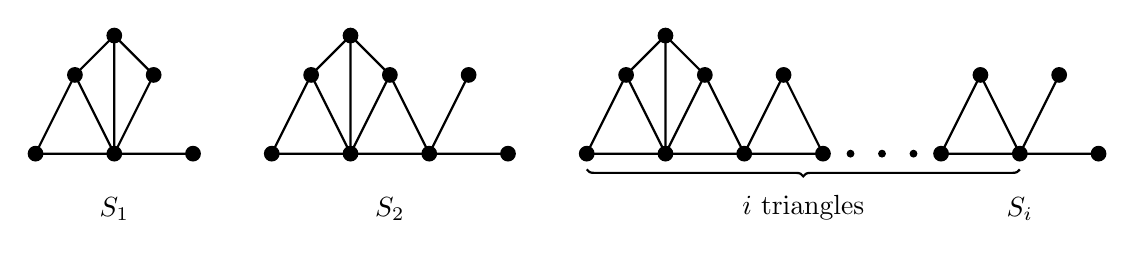
\begin{tikzpicture}[scale=1]
\def\ver{0.1} %size of a vertex
\def\x{1}

\def\xa{0}
\def\ya{0}

\def\xb{0}
\def\yb{0}

\def\xc{4}
\def\yc{0}

\def\xd{9}
\def\yd{0}


%graph S_1
\path[fill] (\xb+1,\yb) circle (\ver);
\path[fill] (\xb+2,\yb) circle (\ver);
\path[fill] (\xb+3,\yb) circle (\ver);
\path[fill] (\xb+2,\yb+1.5) circle (\ver);
\path[fill] (\xb+1.5,\yb+1) circle (\ver);
\path[fill] (\xb+2.5,\yb+1) circle (\ver);

\draw[thick] (\xb+1,\yb)--(\xb+2,\yb)--(\xb+3,\yb)
(\xb+1,\yb)--(\xb+1.5,\yb+1)--(\xb+2,\yb)--(\xb+2.5,\yb+1)
--(\xb+2,\yb+1.5)--(\xb+2,\yb)
(\xb+1.5,\yb+1)--(\xb+2,\yb+1.5);

\node (1) at (\xb+2,\yb-0.7) {$S_1$};



%graph S_2
\path[fill] (\xc,\yc) circle (\ver);
\path[fill] (\xc+1,\yc) circle (\ver);
\path[fill] (\xc+2,\yc) circle (\ver);
\path[fill] (\xc+3,\yc) circle (\ver);
\path[fill] (\xc+0.5,\yc+1) circle (\ver);
\path[fill] (\xc+1.5,\yc+1) circle (\ver);
\path[fill] (\xc+2.5,\yc+1) circle (\ver);
\path[fill] (\xc+1,\yc+1.5) circle (\ver);


\draw[thick] (\xc,\yc)--(\xc+1,\yc)--(\xc+2,\yc)--(\xc+3,\yc)
(\xc+0.5,\yc+1)--(\xc+1,\yc)--(\xc+1.5,\yc+1)--(\xc+2,\yc)--(\xc+2.5,\yc+1)
(\xc,\yc)--(\xc+0.5,\yc+1)--(\xc+1,\yc+1.5)--(\xc+1.5,\yc+1)
(\xc+1,\yc)--(\xc+1,\yc+1.5);

\node (1) at (\xc+1.5,\yc-0.7) {$S_2$};

%graph S_3
\path[fill] (\xd-1,\yd) circle (\ver);
\path[fill] (\xd-0.5,\yd+1) circle (\ver);
\path[fill] (\xd,\yd) circle (\ver);
\path[fill] (\xd+1,\yd) circle (\ver);
\path[fill] (\xd+2,\yd) circle (\ver);
\path[fill] (\xd+3.5,\yd) circle (\ver);
\path[fill] (\xd+4.5,\yd) circle (\ver);
\path[fill] (\xd+5.5,\yd) circle (\ver);
\path[fill] (\xd+0.5,\yd+1) circle (\ver);
\path[fill] (\xd+1.5,\yd+1) circle (\ver);
\path[fill] (\xd+4,\yd+1) circle (\ver);
\path[fill] (\xd+5,\yd+1) circle (\ver);
\path[fill] (\xd,\yd+1.5) circle (\ver);

\fill (\xd+2.35,\yd) circle (\ver/2);
\fill (\xd+2.75,\yd) circle (\ver/2);
\fill (\xd+3.15,\yd) circle (\ver/2);

\draw[thick] (\xd-1,\yd)--(\xd+2,\yd)
(\xd+3.5,\yd)--(\xd+5.5,\yd)
(\xd-1,\yd)--(\xd-0.5,\yd+1)--(\xd,\yd)--(\xd+0.5,\yd+1)--(\xd+1,\yd)--(\xd+1.5,\yd+1)--(\xd+2,\yd)
(\xd+3.5,\yd)--(\xd+4,\yd+1)--(\xd+4.5,\yd)--(\xd+5,\yd+1)
(\xd-0.5,\yd+1)--(\xd,\yd+1.5)--(\xd+0.5,\yd+1)
(\xd,\yd)--(\xd,\yd+1.5);

\draw[thick,decoration={brace,mirror,raise=0.2cm},decorate] (\xd-1,\yd) -- (\xd+4.5,\yd)
node [pos=0.5,anchor=north,yshift=-0.4cm] {$i$ triangles};

\node (1) at (\xd+4.5,\yd-0.7) {$S_i$};



\end{tikzpicture}
\end{center}
\caption{The class $\mathcal{S}$ \cite{joosCharacterizationMixedUnit2013}.}\label{fig:graphsS}
\end{figure}


\begin{figure}[H]
\begin{center}
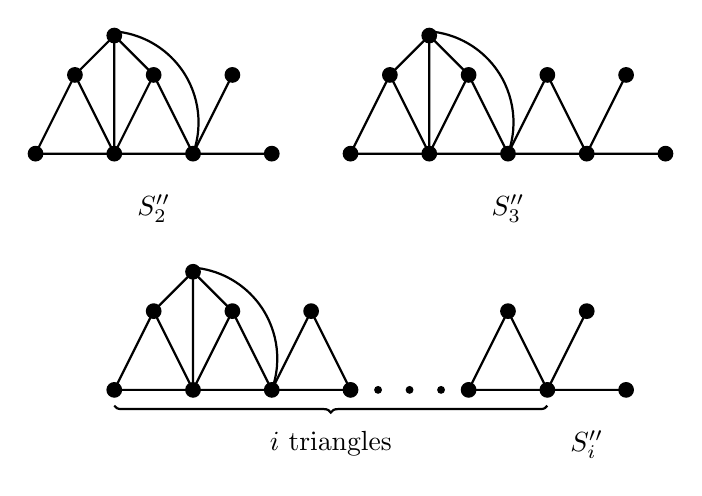
\begin{tikzpicture}[scale=1]
\def\ver{0.1} %size of a vertex
\def\x{1}

\def\xa{2}
\def\ya{-3}

\def\xb{0}
\def\yb{0}

\def\xc{0}
\def\yc{0}

\def\xd{5}
\def\yd{0}

%graph S^2_2
\path[fill] (\xc,\yc) circle (\ver);
\path[fill] (\xc+1,\yc) circle (\ver);
\path[fill] (\xc+2,\yc) circle (\ver);
\path[fill] (\xc+3,\yc) circle (\ver);
\path[fill] (\xc+0.5,\yc+1) circle (\ver);
\path[fill] (\xc+1.5,\yc+1) circle (\ver);
\path[fill] (\xc+2.5,\yc+1) circle (\ver);
\path[fill] (\xc+1,\yc+1.5) circle (\ver);


\draw[thick] (\xc,\yc)--(\xc+1,\yc)--(\xc+2,\yc)--(\xc+3,\yc)
(\xc+0.5,\yc+1)--(\xc+1,\yc)--(\xc+1.5,\yc+1)--(\xc+2,\yc)--(\xc+2.5,\yc+1)
(\xc,\yc)--(\xc+0.5,\yc+1)--(\xc+1,\yc+1.5)--(\xc+1.5,\yc+1)
(\xc+1,\yc)--(\xc+1,\yc+1.5);

\draw[thick] (\xc+2,\yc) arc(-20:85:1.16);

\node (1) at (\xc+1.5,\yc-0.7) {$S_2''$};

%graph S^2_3
\path[fill] (\xd-1,\yd) circle (\ver);
\path[fill] (\xd-0.5,\yd+1) circle (\ver);
\path[fill] (\xd,\yd) circle (\ver);
\path[fill] (\xd+1,\yd) circle (\ver);
\path[fill] (\xd+2,\yd) circle (\ver);
\path[fill] (\xd+3,\yd) circle (\ver);
\path[fill] (\xd+0.5,\yd+1) circle (\ver);
\path[fill] (\xd+1.5,\yd+1) circle (\ver);
\path[fill] (\xd+2.5,\yd+1) circle (\ver);
\path[fill] (\xd,\yd+1.5) circle (\ver);


\draw[thick] (\xd-1,\yd)--(\xd+3,\yd)
(\xd-1,\yd)--(\xd-0.5,\yd+1)--(\xd,\yd)--(\xd+0.5,\yd+1)--(\xd+1,\yd)--(\xd+1.5,\yd+1)--(\xd+2,\yd)--(\xd+2.5,\yd+1)
(\xd-0.5,\yd+1)--(\xd,\yd+1.5)--(\xd+0.5,\yd+1)
(\xd,\yd)--(\xd,\yd+1.5);

\draw[thick] (\xd+1,\yd) arc(-20:85:1.16);

\node (1) at (\xd+1,\yd-0.7) {$S_3''$};

%graph S_i''
\path[fill] (\xa-1,\ya) circle (\ver);
\path[fill] (\xa,\ya) circle (\ver);
\path[fill] (\xa+1,\ya) circle (\ver);
\path[fill] (\xa+2,\ya) circle (\ver);
\path[fill] (\xa+3.5,\ya) circle (\ver);
\path[fill] (\xa+4.5,\ya) circle (\ver);
\path[fill] (\xa+5.5,\ya) circle (\ver);
\path[fill] (\xa-0.5,\ya+1) circle (\ver);
\path[fill] (\xa+0.5,\ya+1) circle (\ver);
\path[fill] (\xa+1.5,\ya+1) circle (\ver);
\path[fill] (\xa+4,\ya+1) circle (\ver);
\path[fill] (\xa+5,\ya+1) circle (\ver);
\path[fill] (\xa,\ya+1.5) circle (\ver);


\draw[thick] (\xa-1,\ya)--(\xa+2,\ya)
(\xa+3.5,\ya)--(\xa+5.5,\ya)
(\xa-1,\ya)--(\xa-0.5,\ya+1)--(\xa,\ya)--(\xa+0.5,\ya+1)--(\xa+1,\ya)--(\xa+1.5,\ya+1)--(\xa+2,\ya)
(\xa+3.5,\ya)--(\xa+4,\ya+1)--(\xa+4.5,\ya)--(\xa+5,\ya+1)
(\xa-0.5,\ya+1)--(\xa,\ya+1.5)--(\xa+0.5,\ya+1)
(\xa,\ya)--(\xa,\ya+1.5);

\draw[thick] (\xa+1,\ya) arc(-20:85:1.16);

\node (1) at (\xa+5,\ya-0.7) {$S_i''$};

\fill (\xa+2.35,\ya) circle (\ver/2);
\fill (\xa+2.75,\ya) circle (\ver/2);
\fill (\xa+3.15,\ya) circle (\ver/2);

\draw[thick,decoration={brace,mirror,raise=0.2cm},decorate] (\xa-1,\ya) -- (\xa+4.5,\ya)
node [pos=0.5,anchor=north,yshift=-0.4cm] {$i$ triangles};


\end{tikzpicture}
\end{center}
\caption{The class $\mathcal{S}''$. \cite{joosCharacterizationMixedUnit2013}}\label{fig:graphsSS}
\end{figure}


\begin{figure}
\begin{center}
  \begin{scaletikzpicturetowidth}{\textwidth}
  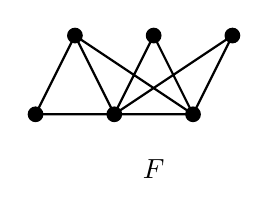
\begin{tikzpicture}[scale=1]
    \def\ver{0.1} %size of a vertex
    \def\x{1}

    \def\xa{0}
    \def\ya{0}

    %G_1
    \path[fill] (\xa+1,\ya) circle (\ver);
    \path[fill] (\xa+2,\ya) circle (\ver);
    \path[fill] (\xa+0.5,\ya+1) circle (\ver);
    \path[fill] (\xa+1.5,\ya+1) circle (\ver);
    \path[fill] (\xa+2.5,\ya+1) circle (\ver);
    \fill (\xa,\ya) circle (\ver);

    \draw[thick] (\xa+1,\ya)--(\xa+2,\ya)
    (\xa+1,\ya)--(\xa+0.5,\ya+1)--(\xa+2,\ya)
    (\xa+1,\ya)--(\xa+2.5,\ya+1)--(\xa+2,\ya)
    (\xa+1,\ya)--(\xa+1.5,\ya+1)--(\xa+2,\ya)
    (\xa+1,\ya)--(\xa,\ya)--(\xa+0.5,\ya+1);

    \node (1) at (\xa+1.5,\ya-0.7) {$F$};

\end{tikzpicture}
\end{scaletikzpicturetowidth}
\end{center}
\caption{The graph $F$. \cite{joosCharacterizationMixedUnit2013}}\label{fig:graphF}
\end{figure}

\begin{figure}[t]
\begin{center}
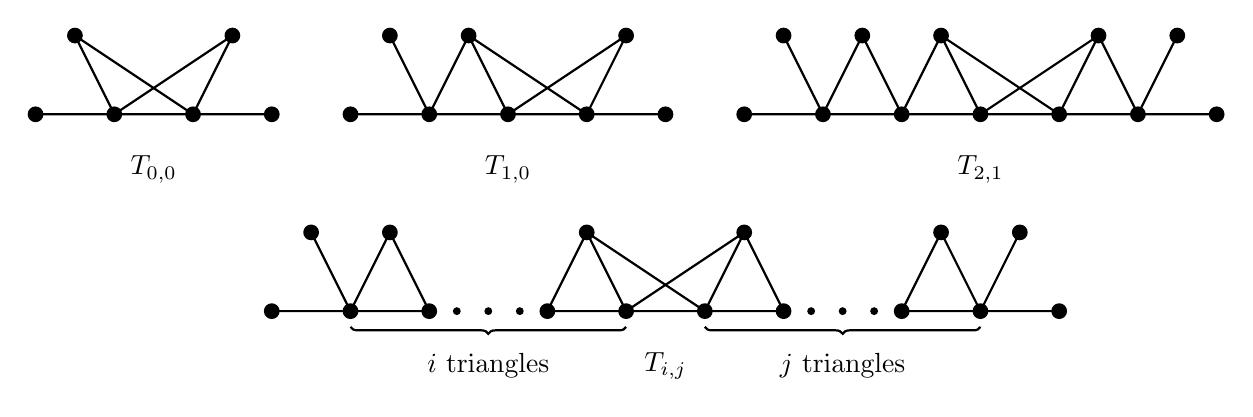
\begin{tikzpicture}[scale=1]
\def\ver{0.1} %size of a vertex
\def\x{1}

\def\xa{0}
\def\ya{0}

\def\xb{4}
\def\yb{0}

\def\xc{9}
\def\yc{0}

\def\xd{3}
\def\yd{-2.5}

%graph T_{0,0}
\path[fill] (\xa,\ya) circle (\ver);
\path[fill] (\xa+1,\ya) circle (\ver);
\path[fill] (\xa+2,\ya) circle (\ver);
\path[fill] (\xa+3,\ya) circle (\ver);
\path[fill] (\xa+0.5,\ya+1) circle (\ver);
\path[fill] (\xa+2.5,\ya+1) circle (\ver);

\draw[thick] (\xa,\ya)--(\xa+3,\ya)
(\xa+1,\ya)--(\xa+0.5,\ya+1)--(\xa+2,\ya)
(\xa+1,\ya)--(\xa+2.5,\ya+1)--(\xa+2,\ya);

\node (1) at (\xa+1.5,\ya-0.7) {$T_{0,0}$};

%graph T_{1,0}
\path[fill] (\xb,\yb) circle (\ver);
\path[fill] (\xb+1,\yb) circle (\ver);
\path[fill] (\xb+2,\yb) circle (\ver);
\path[fill] (\xb+3,\yb) circle (\ver);
\path[fill] (\xb+4,\yb) circle (\ver);
\path[fill] (\xb+0.5,\yb+1) circle (\ver);
\path[fill] (\xb+1.5,\yb+1) circle (\ver);
\path[fill] (\xb+3.5,\yb+1) circle (\ver);

\draw[thick] (\xb,\yb)--(\xb+4,\yb)
(\xb+0.5,\yb+1)--(\xb+1,\yb)--(\xb+1.5,\yb+1)--(\xb+2,\yb)--(\xb+3.5,\yb+1)
--(\xb+3,\yb)--(\xb+1.5,\yb+1);

\node (1) at (\xb+2,\yb-0.7) {$T_{1,0}$};

%graph T_{2,1}
\path[fill] (\xc,\yc) circle (\ver);
\path[fill] (\xc+1,\yc) circle (\ver);
\path[fill] (\xc+2,\yc) circle (\ver);
\path[fill] (\xc+3,\yc) circle (\ver);
\path[fill] (\xc+4,\yc) circle (\ver);
\path[fill] (\xc+5,\yc) circle (\ver);
\path[fill] (\xc+6,\yc) circle (\ver);
\path[fill] (\xc+0.5,\yc+1) circle (\ver);
\path[fill] (\xc+1.5,\yc+1) circle (\ver);
\path[fill] (\xc+2.5,\yc+1) circle (\ver);
\path[fill] (\xc+4.5,\yc+1) circle (\ver);
\path[fill] (\xc+5.5,\yc+1) circle (\ver);

\draw[thick] (\xc,\yc)--(\xc+6,\yc)
(\xc+0.5,\yc+1)--(\xc+1,\yc)--(\xc+1.5,\yc+1)--(\xc+2,\yc)--(\xc+2.5,\yc+1)--(\xc+3,\yc)--(\xc+4.5,\yc+1)
(\xc+5.5,\yc+1)--(\xc+5,\yc)--(\xc+4.5,\yc+1)--(\xc+4,\yc)--(\xc+2.5,\yc+1);

\node (1) at (\xc+3,\yc-0.7) {$T_{2,1}$};

%graph T_{i,j}
\path[fill] (\xd,\yd) circle (\ver);
\path[fill] (\xd+1,\yd) circle (\ver);
\path[fill] (\xd+2,\yd) circle (\ver);
\path[fill] (\xd+3.5,\yd) circle (\ver);
\path[fill] (\xd+4.5,\yd) circle (\ver);
\path[fill] (\xd+5.5,\yd) circle (\ver);
\path[fill] (\xd+6.5,\yd) circle (\ver);
\path[fill] (\xd+8,\yd) circle (\ver);
\path[fill] (\xd+9,\yd) circle (\ver);
\path[fill] (\xd+10,\yd) circle (\ver);
\path[fill] (\xd+0.5,\yd+1) circle (\ver);
\path[fill] (\xd+1.5,\yd+1) circle (\ver);
\path[fill] (\xd+4,\yd+1) circle (\ver);
\path[fill] (\xd+6,\yd+1) circle (\ver);
\path[fill] (\xd+8.5,\yd+1) circle (\ver);
\path[fill] (\xd+9.5,\yd+1) circle (\ver);

\draw[thick] (\xd,\yd)--(\xd+2,\yd)
(\xd+3.5,\yd)--(\xd+6.5,\yd)
(\xd+8,\yd)--(\xd+10,\yd)
(\xd+0.5,\yd+1)--(\xd+1,\yd)--(\xd+1.5,\yd+1)--(\xd+2,\yd)
(\xd+8,\yd)--(\xd+8.5,\yd+1)--(\xd+9,\yd)--(\xd+9.5,\yd+1)
(\xd+3.5,\yd)--(\xd+4,\yd+1)--(\xd+4.5,\yd)
(\xd+5.5,\yd)--(\xd+6,\yd+1)--(\xd+6.5,\yd)
(\xd+4,\yd+1)--(\xd+5.5,\yd)
(\xd+6,\yd+1)--(\xd+4.5,\yd);

\fill (\xd+2.35,\yd) circle (\ver/2);
\fill (\xd+2.75,\yd) circle (\ver/2);
\fill (\xd+3.15,\yd) circle (\ver/2);

\fill (\xd+6.85,\yd) circle (\ver/2);
\fill (\xd+7.25,\yd) circle (\ver/2);
\fill (\xd+7.65,\yd) circle (\ver/2);

\draw[thick,decoration={brace,mirror,raise=0.2cm},decorate] (\xd+1,\yd) -- (\xd+4.5,\yd)
node [pos=0.5,anchor=north,yshift=-0.4cm] {$i$ triangles};

\draw[thick,decoration={brace,mirror,raise=0.2cm},decorate] (\xd+5.5,\yd) -- (\xd+9,\yd)
node [pos=0.5,anchor=north,yshift=-0.4cm] {$j$ triangles};


\node (1) at (\xd+5,\yd-0.7) {$T_{i,j}$};

\end{tikzpicture}
\end{center}
\caption{The class $\mathcal{T}$. \cite{joosCharacterizationMixedUnit2013}}\label{fig:graphsT}
\end{figure}


\section{Unfettered unit interval graphs}
\label{sec:UUIG}

In this section we detail the properties of unfettered \emph{\index{unfettered unit interval graphs}}.
An unfettered unit interval graph can be defined as an unit interval graph such that for every touching endpoints we can chose either if they are adjacent or not. We remark that by definition, every unit interval graph is feasible in UUIG. This class is a minimal superclass of TSG, \textit{i.e.} TSG $\subsetneq$ UUIG.

This class has a characterization by levels done by Hayashi \textit{et al.} where levels are used. A \emph{level structure} of a graph $G = (V,E)$ is a partition $L = \{L_i : i \in [1,t]\}$ of $V$ such that

$$v \in L_k \Rightarrow N(v) \subseteq L_{k-1} \cup L_{k} \cup L_{k+1}$$

where $L_0 = L_{t+1} = \varnothing$.

\begin{theorem}[Hayashi et al. \cite{hayashiThinStripGraphs2017}]
  \label{theo:uuig_char}
  A graph $G$ is an unfettered unit interval graph if and only if it has a level structure where each level is a clique.
\end{theorem}

\proof{
We begin by proving the if-part. Let $G$ be a graph with levels $L_1, \dots, L_t$ where every level is a clique. For every vertex $v \in L_i$, we assign an interval $[i-1, i]$. We see that every interval within a level is in the same position, so they are all adjacent. Then, for $L_i$ we have its adjacent levels $L_{i-1}$ and $L_{i+1}$. The right endpoints of the intervals $L_{i-1}$ match the left endpoints of $L_i$. On the other side, the left endpoints of $L_{i+1}$ match the right endpoints of $L_i$. As we know, we can chose whether the endpoints touch or not between levels. This will construct its respective UUIG.

Now we prove the only-if. Let $G$ be a UUIG and $I(v)$ the interval representation of $v \in V(G)$ and $\ell(I(v))$ the left side of an interval. Let $I'(v) = [\floor{\ell(I(v))},\floor{\ell(I(v))}+1]$. This gives us exactly the same graph because the following holds:

\begin{equation}
\begin{split}
  \ell(I(v)) - \ell(I(v)) \leqslant 1 \Rightarrow & \floor{\ell(I(v))} - \floor{\ell(I(v))} \leqslant 1 \\
  \ell(I(v)) - \ell(I(v)) \geqslant 1 \Rightarrow & \floor{\ell(I(v))} - \floor{\ell(I(v))} \geqslant 1
\end{split}
\end{equation}

We can have a partition $L_i = \{v : \ell(I'(v)) = i\}$ where every $L_i$ is a clique. Also, this partition is a level structure because the endpoints of $L_i$ meet the endpoints of $L_{i-1}$ and $L_{i+1}$. \qed

}

We can clearly see that MUIG $\in$ UUIG. However, we still have to see what is the location of UUIG in the higher graph classes hierarchy:

\begin{prop}
  UUIG $\subset$ co-comparability.
\end{prop}

\proof{This proposition is equivalent to say that if a graph $G$ is a UUIG, then it also has a spanning order.

For each vertex of a partition $L_k$ of UUIG (Theorem \ref{theo:uuig_char}) we assign arbitrarily a number $i \in \{\max(V(L_{k-1}))+1, \dots, \max(V(L_{k-1}))+|V(L_k)|+1\}$; intuitively, we assign every available number from the beginning in increasing order ($|V(L_1)|$ first numbers on the first partition and consecutively).

Because we know that each partition $L_k$ is a clique, we can say that for each three vertices $u < v < w$, if $vw \in E \Rightarrow uv\in E\  \text{or} \ vw\in E$. We know this because given $u \in L_i$ and $w \in L_j$: if $uw\in E$ it means that levels $L_i$ and $L_j$ are adjacent, which means that $v\in L_i$ or $v\in L_j$ so $v$ will be adjacent either to $u$ or $w$. This is a spanning order. \qed
}\\

If we recall the characterization of MUIG in section \ref{sec:muig_char}, we can see that every forbidden graph of MUIG is an
UUIG (except for $\mathcal{R}$); which means that they are also co-comparability graphs.

In the other hand, we can find a graph in UUIG that is not an UDG. This theorem will be used in Chapter \ref{chap:thinDef}.

\begin{figure}
  \begin{center}
\begin{scaletikzpicturetowidth}{\textwidth}
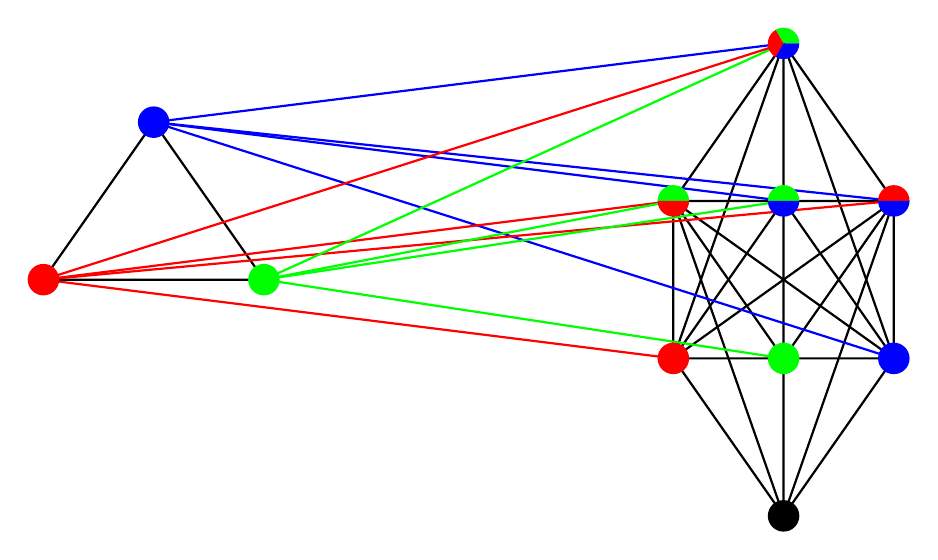
\begin{tikzpicture}[scale=2]
\def\xa{-2}
\def\ya{0.5}
\def\xb{2}

\def\ver{0.1} %size of a vertex


% LEVEL 1 edges
\draw[thick] (\xa,\ya) -- (\xa+0.7,\ya-1) -- (\xa-0.7,\ya-1) -- (\xa, \ya);

% LEVEL 2 edges
\draw[thick] (\xb,-2) -- (\xb-0.7,-1) -- (\xb-0.7,0) -- (\xb, 1) -- (\xb+0.7,0) -- (\xb+0.7,-1) -- (\xb,-2) -- (\xb, 1);

\draw[thick] (\xb-0.7,-1) -- (\xb+0.7,0) -- (\xb-0.7,0) -- (\xb+0.7, -1) -- (\xb-0.7,-1);

\draw[thick] (\xb, 1) -- (\xb-0.7, -1) -- (\xb, 0);
\draw[thick] (\xb, 1) -- (\xb+0.7, -1) -- (\xb, 0);
\draw[thick] (\xb, -2) -- (\xb+0.7, 0) -- (\xb, -1);
\draw[thick] (\xb, -2) -- (\xb-0.7, 0) -- (\xb, -1);


% between levels
\draw[thick, color=blue] (\xa, \ya) -- (\xb+0.7, -1);
\draw[thick, color=green] (\xa+0.7,\ya-1) -- (\xb, -1);
\draw[thick, color=red] (\xa-0.7,\ya-1) -- (\xb-0.7, -1);

\draw[thick, color=blue] (\xa,\ya) -- (\xb+0.7, 0);
\draw[thick, color=blue] (\xa,\ya) -- (\xb, 0);
\draw[thick, color=red] (\xa-0.7,\ya-1) -- (\xb-0.7, 0);
\draw[thick, color=red] (\xa-0.7,\ya-1) -- (\xb+0.7, 0);
\draw[thick, color=green] (\xa+0.7,\ya-1) -- (\xb-0.7, 0);
\draw[thick, color=green] (\xa+0.7,\ya-1) -- (\xb, 0);

\draw[thick, color=blue] (\xa, \ya) -- (\xb, 1);
\draw[thick, color=green] (\xa+0.7,\ya-1) -- (\xb, 1);
\draw[thick, color=red] (\xa-0.7,\ya-1) -- (\xb, 1);

% LEVEL 1 vertices

\fill[color=blue]  (\xa,\ya)      circle (\ver);
\fill[color=green]    (\xa+0.7,\ya-1)   circle (\ver);
\fill[color=red]   (\xa-0.7,\ya-1)  circle (\ver);

% LEVEL 2 vertices

\fill (\xb,-2) circle (\ver);

\fill[color=blue] (\xb+0.7,-1) circle (\ver);
\fill[color=red] (\xb-0.7,-1) circle (\ver);
\fill[color=green] (\xb,-1) circle (\ver);

\fill[color=green] (\xb,0) -- (\xb+\ver, 0) arc (0:180:\ver) -- (\xb, 0);
\fill[color=blue] (\xb,0) -- (\xb-\ver, 0) arc (180:360:\ver) -- (\xb, 0);

\fill[color=red] (\xb + 0.7,0) -- (\xb + 0.7+\ver, 0) arc (0:180:\ver) -- (\xb + 0.7, 0);
\fill[color=blue] (\xb + 0.7,0) -- (\xb + 0.7-\ver, 0) arc (180:360:\ver) -- (\xb + 0.7, 0);

\fill[color=green] (\xb - 0.7,0) -- (\xb - 0.7+\ver, 0) arc (0:180:\ver) -- (\xb - 0.7, 0);
\fill[color=red] (\xb - 0.7,0) -- (\xb - 0.7-\ver, 0) arc (180:360:\ver) -- (\xb - 0.7, 0);


\fill[color=green] (\xb,1) -- (\xb+\ver, 1) arc (0:120:\ver) -- (\xb, 1);
\fill[color=red] (\xb,1) -- (\xb - 0.5*\ver, 1 + 0.86*\ver) arc (120:240:\ver) -- (\xb, 1);
\fill[color=blue] (\xb,1) -- (\xb - 0.5*\ver, 1 - 0.86*\ver) arc (240:360:\ver) -- (\xb, 1);

\end{tikzpicture}
\end{scaletikzpicturetowidth}
\end{center}
\caption{Representation of $T$ with three vertices in the first level instead of four where every level is a clique. The colors represent the three vertices of the first level. The multicolored vertices represent sets of the vertices in the first level.}
\label{fig:udg3}
\end{figure}

\begin{figure}
\centering

\begin{scaletikzpicturetowidth}{\textwidth}
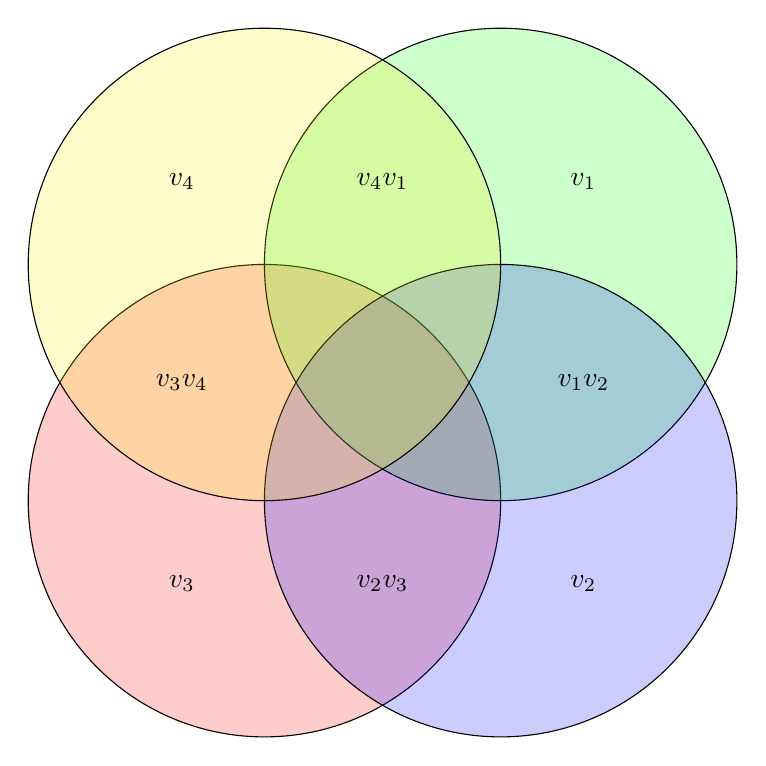
\begin{tikzpicture}[scale=1.5]

\draw[fill=red, fill opacity=0.2]  (-1,-1) circle [radius=2];
\draw[fill=green, fill opacity=0.2]  (1,1) circle [radius=2];
\draw[fill=blue, fill opacity=0.2]  (1,-1) circle [radius=2];
\draw[fill=yellow, fill opacity=0.2]  (-1,1) circle [radius=2];

\draw[color=black] (1.7,1.7) node {$v_1$};
\draw[color=black] (1.7,0) node {$v_1v_2$};
\draw[color=black] (1.7,-1.7) node {$v_2$};
\draw[color=black] (0,-1.7) node {$v_2v_3$};
\draw[color=black] (-1.7,-1.7) node {$v_3$};
\draw[color=black] (-1.7,0) node {$v_3v_4$};
\draw[color=black] (-1.7,1.7) node {$v_4$};
\draw[color=black] (0,1.7) node {$v_4v_1$};

\end{tikzpicture}
\end{scaletikzpicturetowidth}
\caption{A disk Venn diagram of four sets. Each circle of color represent a set. You may notice that some subsets are not represented here (\textit{e.g.} $v_2v_4$ or $v_1v_3$). So a disk that touches $v_4$ and $v_2$ in this representation is not possible without intersecting also $v_3$ or $v_1$.}
\label{fig:uuigudg}
\end{figure}

\begin{theorem}[Hayashi et al. \cite{hayashiThinStripGraphs2017}]
  \label{theo:uuigudg}
  UUIG $\neq$ UDG.
\end{theorem}

\begin{proof}
  We can define $T = (L_1\cup L_2, E)$ a UUIG with two levels $L_1=\{v_1, v_2, v_3, v_4\}$ and $L_2=\powerset(L_1)$ and $E = \binom{L_1}{2} \cup \binom{L_2}{2} \cup \{vw: w\in L_2, v\in w\}$. For a better visualisation, you can find in Figure \ref{fig:udg3} the representation as an UDG in the case where $L_1 = \{v_1, v_2, v_3\}$.

  We can see the UDG representation of $G$ as a Venn diagram of four disks ($L_1$) where there is a disk of $L_2$ that intersects only with its subset associated. We know by instance that a Venn diagram cannot be constructed with disks if the number of sets is bigger than four \cite{vennDiagrammaticMechanicalRepresentation1880} as you can see in Figure \ref{fig:uuigudg}. Thus, there will be at least one disk that is not able to intersect with its associated subset because there is at least one subset that is not representable by a disk Venn Diagram. Which means that $G \notin$ UDG.
\end{proof}

\begin{figure}
  \begin{center}
\begin{scaletikzpicturetowidth}{\textwidth}
\begin{tikzpicture}[scale=1]
  \node (1) [draw, rounded rectangle] {co-comparability graphs};
  \node (2) [below=of 1, draw, rounded rectangle] {unfettered unit interval graphs};
  \node (3) [below=of 2, draw, rounded rectangle] {mixed unit interval graphs};
  \node (4) [below=of 3, draw, rounded rectangle] {unit interval graphs};
  \draw[<-] (1) edge (2) (2) edge (3) (3) edge (4);
\end{tikzpicture}
\end{scaletikzpicturetowidth}
\end{center}
\caption{Extension of the graph classes diagram from Figure \ref{fig:hierarchyMUIG} with \emph{UUIG}.}
\label{fig:hierarchyUUIG}
\end{figure}


\subsection{Recognition}

As we mentioned in the previous section, UUIG is a class of graphs very relevant to define TSG and that is why we are interested in knowing how this class of graphs is recognized.

\begin{lemma}
  Let $G$ be a connected UUIG with a level structure with levels $L_1,\dots,L_n$. $G\setminus L_i$ is a graph where each connected component is also an UUIG and the number of connected components is not bigger than two.
\end{lemma}

\proof{By definition for a graph with a level structure, if $v\in L_i$, $N(v) = L_{i-1} \cup L_{i} \cup L_{i+1}$. This said, if we delete a level $L_i$, $L_{i-1}$ and $L_{i+1}$ are disconnected, but they are still connected to the other consecutive levels ($L_{i-1}$ is connected to $L_{i-2}$, which is connected to $L_{i-3}$... and viceversa with $L_{i+1}$).

And because a level is only adjacent to two other levels, we only have two connected components, only one if $L_i = L_1$ or $L_i = L_n$.\qed}\\

By this lemma we can suppose that the input graph $G$ is a connected graph. This observation reduces the complexity of the problem for a graph $G$ from $\mathcal{O}(f(|V(G)|)$ to $\mathcal{O}(f(|V(H)|))$ where $H \subseteq G$ the biggest component of $G$.

\begin{theorem}
  UUIG recognition is in $\mathcal{NP}$.
\end{theorem}

\proof{The UUIG recognition of a graph $G$ is in $\mathcal{NP}$ because we can build a \emph{polynomial time verifier} that takes a level structure of $G$ and check whether each level is a clique or not. Viceversa, we can build another one that takes a partition and check whether each clique is a level of a level structure. \qed}

Future work on the recognition of unfettered unit interval graphs would be to adapt this algorithm to avoid combinatorial complexity. In our case we are interested in seeing the recognition of UUIG for unit disk graphs. We know that the CLIQUE problem is in $\mathcal{P}$ for unit disk graphs \cite{CLARK1990165} and the first hypothesis was that given an UUIG $G$, at least one level of $G$ is a maximal clique of the graph. Nevertheless, we have a counterexample in $T_{0,0}$ (Fig. \ref{fig:graphsT}) where the levels of the graph are $\{K_1, K_2, K_2, K_1\}$ while $\omega(T_{0,0}) = 3$.

\begin{obs}
  Given an UUIG $G$, a level of $G$ does not have to be necessarily a maximal clique.
\end{obs}
